\begin{figure}[htbp]
\centering
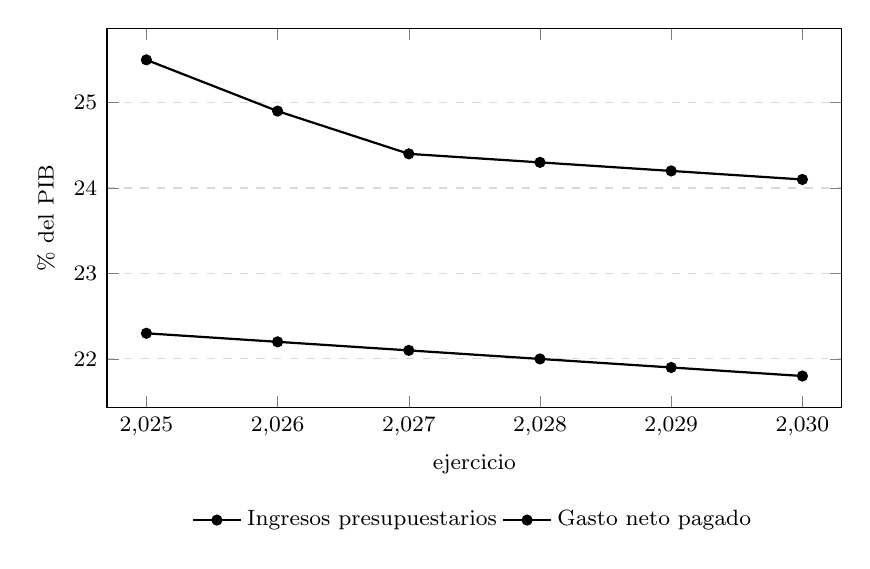
\begin{tikzpicture}
\begin{axis}[
  width=0.9\textwidth, height=6.4cm,
  xlabel={ejercicio}, ylabel={\% del PIB},
  legend style={font=\footnotesize, at={(0.5,-0.24)}, anchor=north,
                 legend columns=-1, draw=none},
  tick label style={font=\footnotesize},
  label style={font=\footnotesize},
  ymajorgrids=true, grid style={dashed, gray!30},
  enlarge x limits=0.06,
  xtick=data,
]
\addplot[mark=*, mark size=1.6pt, thick] coordinates {(2025,22.3) (2026,22.2) (2027,22.1) (2028,22.0) (2029,21.9) (2030,21.8)};
\addlegendentry{Ingresos presupuestarios}
\addplot[mark=*, mark size=1.6pt, thick] coordinates {(2025,25.5) (2026,24.9) (2027,24.4) (2028,24.3) (2029,24.2) (2030,24.1)};
\addlegendentry{Gasto neto pagado}
\end{axis}
\end{tikzpicture}
\caption{Ingresos y gasto neto en el escenario oficial, 2025--2030}
\label{fig:F2_1}
\par\vspace{2pt}\footnotesize Fuente: elaboración propia del ITED con información de la SHCP, CGPE 2025, Anexo III.2, p.\textasciitilde{}85. La brecha se cierra bajando el gasto, no subiendo el ingreso. El CGPE 2025 se publicó sin capa de texto; las cifras se leyeron de la página renderizada y se validaron por identidad contable.
\end{figure}
